%% This document gives an example on how to use the ntnumasterthesis
%% LaTeX document class.

%% Use short name MACS, MIS, CIMET, MTDMT, MIXD or MIS
%% Language english or norsk
%% b5paper with oneside or twoside, you can set A4 if you want but you submit in b5

%% If you want print with the heading material on a4 paper you can use this format
%% \documentclass[MACS,english,a4paper,oneside,12pt]{ntnuthesis/ntnuthesis}

%% with the change to using DAIM we have a new option.
\documentclass[MACS,english,DAIM]{ntnuthesis/ntnuthesis}

\usepackage[T1]{fontenc}
\usepackage[utf8]{inputenc}     % For utf8 encoded .tex files allows norwegian characters in the files. This can be dangerous if you change to a differnt editor.
%\usepackage[pdftex]{graphicx, hyperref}   % For cross references in pdf
\usepackage{graphicx}
\usepackage{hyperref}   % For cross references in pdf


\usepackage{color}              % For colouring text
\hypersetup{colorlinks=true,
		linkcolor=blue,          % color of internal links (change box color with linkbordercolor)
    citecolor=blue,        % color of links to bibliography
    filecolor=blue,      % color of file links
    urlcolor=blue           % color of external links
		}
\usepackage{csvsimple}  % for simple table reading and display
\usepackage{url}

% Set to true ONLY if using Harvard citation style
\newboolean{HarvardCitations}
\setboolean{HarvardCitations}{false} % false for computer science, true for interaction design and harvard style


\ifthenelse{\boolean{HarvardCitations}}{%
	\usepackage{natbib} % for Harvard names as citations.
}{%
	\usepackage[numbers]{natbib} % for Vancover numbers in bibliography
}



\begin{document}

% !TEX root = ../Masters.tex
% for students submitting in the DAIM system this information will not be used.
% their is an option for DAIM submission which removes this information and checks it is B5.
% Removing the DAIM option on the document type will use this material.

\setthesistitle{Using L-systems to generate aesthetic plant offspring}
%\setthesisshorttitle{Example Masters Thesis} % a short version for the page headers if your normal title is too long to fit
\setthesisauthor{Magnus Bjerke Vik}
\setthesissupervisor{Mariusz Nowostawski}
%\setthesissupervisorA{Prof. Jon Yngve Hardeberg}  % if you have a second supervisor add it like this


\nmtkeywords{Thesis, Latex, Template, IMT}
%\nmtdesc{This is the short description of a masters thesis}


\setthesisdate{01-06-2017}
\setthesisyear{2017}



%for CIMET theses you need to see all of these as well

%\setthesiscampus{Gj\o{}vik}
%\setthesisHostInstitution{\NTNU}
%\setthesisHostInstitution{University of Eastern Finland}
%\setthesisHostInstitution{Universit\'e Jean Monnet Saint-Etienne}

%\setthesisjuryA{} %jury names
%\setthesisjuryB{} %jury names
%\setthesisjuryC{} %jury names
%\setthesisjuryD{} %jury names
 % this is the file which contains all the details about your thesis
\makefrontpages % make the frontpages
%this is the intro to the thesis
%\thesistitlepage % make the ordinary titlepage
\hypersetup{pageanchor=false}
%\include{summary}

\chapter*{Preface}
Here, you give a brief introduction to your work. What it is (e.g., a Master's thesis in AIMT at NTNU, when it was carried out (e.g., during the autumn semester of 2021). If the project has been carried out with a company, you should mention this and also describe the cooperation with the company. You may also describe how the idea to the project was brought up.

You should also specify the assumed background of the readers of this report (who are you writing for).\\[2cm]

%\begin{center}
%\thesiscampus, 
\thesisdate \\[1pc]
\\[1pc]
%\thesisauthor
%\end{center}

% !TEX root = ../Masters.tex
\chapter*{Acknowledgment}
I would like to thank my supervisor, Mariusz Nowostawski, for helping me with his insight, interesting ideas and discussions.
I would also like to thank my girlfriend, Merete Nilssen Ringen, for her support and grammatical fixes.
Finally I would like to thank my classmates for making the process of writing the thesis a bit more fun.

% I would like to thank the following persons for their great help during \ldots
%
% If the project has been carried out in cooperation with an external partner (e.g., a company), you should acknowledge the contribution and give thanks to the involved persons.
%
% You should also acknowledge the contributions made by your supervisor(s).

\begin{flushright}
M.B.V.\\[1pc]
\end{flushright}


% !TEX root = ../Masters.tex
\chapter*{Abstract}

This thesis explores how to improve L-system plant generation using \glspl{EA}.
The plants should be aesthetically pleasing, varied, and have the ability to be combined with other plants.

Previous work has shown that simple \glspl{D0L-system}, \glspl{PD0L-system} and \glspl{PDIL-system} can be evolved using \glspl{EA} both autonomously and interactively.
The \gls{L-system} grammar used is simple, restricting the possible solutions.
Additionally often only parts of the grammar is represented in the genotype that is used in the \gls{EA}, thus limiting the evolution.

More complex \glspl{L-system} are required to generate aesthetically pleasing and varied plants, but this also complicates the generator and therefore also the evolution.
To mitigate this issue, \gls{DGEL} is introduced and implemented.
It is based on \gls{GE} of \glspl{L-system}, but introduces a grammar distribution to control what parts of the grammar that should have a higher priority.
\Gls{SA} is used to optimize this grammar distribution so that \gls{DGEL} can produce well performing plants in a more efficient manner.
Additionally, using different optimized grammar distributions could allow for a larger variety of plants, while still keeping the quality up.
Fitness metrics used were both adapted from the reviewed literature and created from scratch to assess the pleasingness of the generated L-system plants.

\Gls{DGEL} was evaluated in three parts: \gls{GE}, \gls{SA} and fitness function.
Plain \gls{GE} was tested against a random brute-force approach to see if it has any benefit.
\Gls{SA}s progress and produced grammar distribution was studied in depth, and its performance was compared in multiple ways using both \gls{GE} and random brute-force approaches.
The fitness metric was compared to human evaluations of generated L-system plants through \gls{AHP} and rank correlation statistics.
Additionally, it was analyzed what factors humans think are important for distinguishing good from bad plants.
\Gls{GE} was found to be superior to brute-force.
\Gls{SA} was found to improve the efficiency of both brute-force and \gls{GE}.
Finally, the fitness function was found to not match the human evaluation, but a small correlation was still present.

The findings suggest that \gls{DGEL} can improve the efficiency of generating L-system plants in a complex space. In a more general sense, the findings suggest that accompanying an EA with a probability distribution, and optimizing it using optimization techniques, can improve its efficiency in complex spaces, allowing for faster searches and more varied solutions.

\hypersetup{pageanchor=false}




\tableofcontents

\hypersetup{pageanchor=true}

% Comment with a percent to remove figures or tables:
\listoffigures
\listoftables

\chapter{Introduction}
\label{chap:introduction}

\section{Topic covered by the project}
In the area of computer graphics and visualization, there is a desire to replicate environments and creatures found in nature in a virtual environment.
All types of environments and creatures are of interests.
Some examples are terrain, mountains, rivers, plants, animals and bacteria.
These can be recreated by manually modeling the specific objects, but to be able to represent the large variations of the objects, this method is tedious and costly.
Another approach to solve this is to procedurally generate the content using procedural content generation (PCG) methods.
This way, digital programs can generate virtually infinite amounts of variations based on a representation and a recipe.

Plants can be generated using L-Systems~\cite{2012Prusinkiewicz}, where their structure is represented as strings of characters in a parallel rewrite system.
Based on actual plants, one may model a virtual plant by creating the rewrite rules and parameters for how the system should be drawn.
Alternatively, it is possible to generate new plant species by using genetic algorithms and natural selection.

\section{Keywords}
L-system, plant, procedural content generation, PCG, genetic algorithm, feature extraction.

\section{Problem description}
\label{sec:ProblemDescription}
% Should add some sources.
Plants can be cross-bred and selected to create offspring with desirable features from multiple species.
For example, most of the species used in agriculture have gone through selection and cross-breeding over several years to yield species that produce a bigger quantity of food and are resistant to deceases and harsh environments.
This can be a long process, taking several hundred of years with gradual improvements, and many combinations do not even work.
To make this process more fun and interesting, a virtual world where people can cross-breed plants can be created.
In this world, cross-breeding is not limited like it is in the real world.
Plants could be combined in ways never possible in the real world.
For example, a user may like both apple trees and Venus flytraps, so they want to combine them into a tree with Venus flytrap mouths that could eat humans.
The problem here is that randomly crossing the representation of different plants may not produce meaningful or interesting offsprings, but rather random creatures that do not satisfy the user.

\section{Justification, motivation and benefit}
Solving this problem will create the foundation for multiple games based on or using cross-breeding of plants.
Additionally, it may be possible to generalize the results to other areas of cross-breeding and PCG, such as breeding animals, or generating levels.
Creating a game based on cross-breeding where the offsprings may be disliked by the users may be catastrophic and result in a game that will not make any revenue.

The results from this research can be used in a game where users may create their own virtual garden, potentially in virtual reality (VR), where they breed the plants they always wanted to see or new surprising species, and have a place outside the busy world to relax and watch their plants grow.
The research results will directly benefit game developers wishing to create games like the one described, and indirectly benefit the PCG research community, other game areas, users of the produced games and companies developing and publishing games.
The game developers and publishers will benefit from more revenue by producing new and interesting games, while users will benefit from new games that fulfill their entertainment and relaxation needs.

\section{Research questions}
The problem described can be summarized in a single research question: How can plant L-systems be combined into offspring that humans find at least as aesthetically pleasing as its parents?
As L-systems can be used to generate various types of shapes, not only plants, ``plant L-systems'' is used as a term meaning L-systems used for generating plants.
To avoid having to reuse the term ``plant L-system'', the term ``L-system'' from this point on mean specifically L-systems to generate plants in the context of the problem.
A hypothesis to this question is that if distinct features from both parents are included in the offspring, the offspring should be at least as pleasing as its parents.
Thus, the initial question can be split into two more specific sub questions: How can L-systems be combined to create offspring with distinct features from both parents, and how aesthetically pleasing are the generated offspring compared to their parents?

To discover how L-systems can be combined with features from both parents, some more knowledge is needed.
First, the L-systems should be able to represent plants both found in nature and not found in nature, as the problem involves combining existing plants into new plants.
Thus a new research question is defined: What types of L-systems are appropriate to represent plants both found in nature and not found in nature?
To combine the L-systems together into offspring with distinct features from both parents, features in an L-systems that appropriately reflect the features found in the produced plants need to be identified.
This gives raise to the question: What are the features of an L-system that can be combined?
Finally, the combination of the features needs to happen, and thus comes the question: How can the features be combined to create offspring that contain distinct features from both parents?

In the end, there is one main research question, and four sub questions that aim to answer the main question.
The questions are listed below.
It is important to notice that these questions can not be answered individually, but as a sequence where the next question depends on the previous.

\begin{description}
    \item[RQ0] How can plant L-systems be combined into offspring that humans find at least as aesthetically pleasing as its parents?
    \begin{description}
        \item[RQ1] What types of L-systems are appropriate to represent plants both found in nature and not found in nature?
        \item[RQ2] What are the features of an L-system that can be combined?
        \item[RQ3] How can the features be combined to create offspring that contain distinct features from both parents?
        \item[RQ4] How aesthetically pleasing are the resulting plants compared to their parents?
    \end{description}
\end{description}

\section{Contribution}
\begin{itemize}
    \item A literature review of L-system representations and features of those representations.
    \item A proposed algorithm for how to combine L-systems while retaining distinct features from both parents.
    \item A software implementation of the algorithm that can take two L-systems and combine them into a new L-system.
    \item An analysis of how well users perceive the combination of plants using the algorithm.
\end{itemize}

\chapter{Plant Representation With L-system}

\section{L-systems}
L-systems was introduced by Lindenmayer in 1968 as a ``theoretical framework for studying the development of simple multicellular organisms''~\cite{Prusinkiewicz2012}, and then later applied to model plants.
An L-system consists of an alphabet, an axiom and a set of production rules.
It is a parallel rewrite system where each letter in the axiom word is rewritten independently based on the production rules.
This happens iteratively, where a new word replaces the previous word each iteration.
A way to draw the plant based on the L-System has to be applied to visualize it.
Prusinkiewicz and Lindemayer summarize multiple research papers into a comprehensive book about L-systems~\cite{Prusinkiewicz2012}.
For a more comprehensive and in-depth explanation of L-systems, refer to this book.

There are also multiple types of L-systems, including discrete, stochastic, context sensitive and parametric~\cite{Prusinkiewicz2012}.
All of these can be combined into one L-system.
A stochastic, context sensitive and parametric L-system (parametric S2L-System) can model all of the other types of L-System by having 100\% probabilities (discrete), no contexts or no parameters, and is thus the most flexible representation.
To be able to generate realistic looking plants with variations per instance, a parametric S2L-system is required.

Discrete context-free L-systems (D0L-systems) are the simplest L-systems, and can be created using edge rewriting, node rewriting, or both~\cite{Prusinkiewicz2012}.
In these systems, there exists one production rule per letter in the alphabet.
By default the productions will produce the same letter as the input (identity).

Stochastic L-systems add a randomness to the generation of the plants.
Each letter in the alphabet may have multiple productions, each with a probability of being selected~\cite{Prusinkiewicz2012}.
This may simulate how different instances of a plant species may look slightly different, thus making the plants look less synthetic when seen together with other plants of the same species.

Context sensitive L-systems add a context to the production rule.
The context can be on either left, right or both sides of the letter.
A production will only be used if the context matches the surrounding letters in the word.
With this, signal propagation can be simulated either upwards or downwards through the plant~\cite{Prusinkiewicz2012}, and more complex plants may be generated.

Parametric L-systems adds parameters to the letters in the words, and conditial rules~\cite{Prusinkiewicz2012}.
The main benefit of using parametric L-systems, is that it can work with rational numbers rather than only integers.
For example, with non-parametric L-systems, extension of a segment can be modeled with the rule $F\rightarrow FF$, or any number of ``F'' in the successor.
In any case, it will only be possible to grow the segment with a multiple of the previous.
For some plants, this is enough, but to model a larger variety of plants, rational numbers are required.
With parametric L-systems, the same rule would be $F(l)\rightarrow F(l*2)$, where $l$ is the length of the segment.
But now it is also possible to grow it at another rate, e.g.\ $F(l)\rightarrow F(l*1.2)$.
Prusinkiewicz and Lindenmayer describe more of the benefits of parametric L-systems~\cite{Prusinkiewicz2012}.

Prusinkiewicz describe L-systems as having three levels of model specification: partial L-systems, L-system schemata, and complete L-systems~\cite{Prusinkiewicz2012}.
The three different levels go from more abstract to more concrete, where partial L-systems specify which structures may result into which new structures (e.g.\ bud becomes a flower), schemata specifies when the different structure switches happen (e.g.\ when the bud becomes a flower), and complete systems specify the geometry of the plant to be visualized (e.g.\ how the bud and the flower should look).
Different methods exist for each level, and which method to use will depend on the type of plant that should be generated.

L-system schemata is of particular interest because there exists multiple methods to use.
The event of a structure resulting into a new structure is called a ``developmental switch''~\cite{Prusinkiewicz2012}.
The timing of the switches need to be controlled by a control mechanism in the system.
There are two classes of these mechanisms: lineage and interaction.
Lineage mechanisms are transferring information from a module to a descendant, while interaction mechanisms exchange information between cells.
Prusinkiewicz and Lindenmayer descibe some of the mechanisms used.
The stochastic mechanism uses a stochastic L-system to apply probabilities to developmental switches.
A table L-system has multiple tables with different rules that can be applied depending on some external factor.
For example, one table can represent summer and another can represent winter, making different switches happen at differnet seasons.
The delay mechanism can delay the developmental switch by a specified number of iterations, for example making a flower bud bloom after a certain amount of iterations.
Accumulation of components uses parametric L-systems to accumulate some parameter until it reaches a threshold causing the switch to happen.
Parametric L-systems can also be used to control development switches with signals, where a signal travels either upwards or downwards through the plant.~\cite{Prusinkiewicz2012}

A popular way to render complete L-systems is the turtle interpretation, where a cursor (the turtle) follows instructions to draw lines, and the alphabet is the set of instructions to use~\cite{Prusinkiewicz2012}.
Turtle interpretation is in its original form simple and can only draw lines on a 2D image, but it has been extended to draw realistic looking plants in 3D~\cite{Prusinkiewicz1988}.
To use the turtle interpretation, extra parameters describing how much the L-system should be expanded and how it should be drawn has to be defined~\cite{Prusinkiewicz2012}.
For example, the number of rewrite iterations, the branching angle, the segment length, and the segment width have to be specified.
This may depend on the plant to be rendered, as some plants might require a more complex set of drawing instructions.

\section{Genetically Evolving L-systems}
Genetic evolution involves crossing genes from parents to create an offspring.
Thus, the research field of L-system genetic evolution is a good starting point for finding out how L-systems can be combined into offspring with distinct features from both parents, potentially providing a basis for answering \textit{RQ2} and \textit{RQ3}.
A set of research papers published between 1995 and 2013 was studied to see what different techniques have been used.

When evolving objects, an evolutionary algorithm (EA) is often used.
EA is composed of a series of steps that will evolve a population over multipe generations based on some criteria.
It begins by generating an initial population of individuals.
Then it evaluates the individuals with a fitness function.
This is then used to select the best individuals to be used for reproduction.
The individuals are then used to create offspring for a new population by using crossover and mutation.
Finally, the new population is evaluated and the steps repeat.
In the context of L-systems, the \textit{object} will be replaced with L-system.

To get a better overview of the EA techniques used for L-systems, the EA has been split into five parts: model, representation, generation, selection, and genetic operators.
The \textit{model} and \textit{representation} are related and sometimes almost equal.
The difference is that the model represents the plant is modelled, while the representation may be a small part of the model or the model represented in a different format.
\textit{Generation} is how the representations are generated, e.g.\ for the initial population, or when replacing parts of an L-system with a new part.
\textit{Selection} is the part of selecting individuals to be used for creating the next generation.
\textit{Genetic operators} are used on the selected individuals to modify the representation by either doing crossover between parents, mutating an offspring, or both.

% From here and below should be moved to Related Work.
%Niklas pioneered artificial evolution of L-systems in 1986. % Can't find copy of paper. Only have one source from another paper. Remove this?
Jacob argues that manually inferring an L-system from a real plant seen in nature is a difficult and tedious task involving several steps~\cite{Jacob1998}.
Some of these steps can be automated using evolutionary algorithms, specifically defining L-systems, comparing the generated plant with the real plant and correcting the L-system based on how it matched.
Based on this, Jacob defines three parts of evolutionary L-system inference: generation functions that create L-systems within some constraints, evaluation functions that measure the fitness of the interpreted L-system, and modification and selection functions that allow editing of L-systems with evolutionary techniques.

To evolve the L-systems, Jacob uses Genetic Programming (GP) techniques introduced by Koza~\cite{Koza1993}.
The difference is that Jacob uses higher-order building blocks for generation and modification of expressions.
A pool of expression patterns is defined that contains several expressions that each are represented in a tree structure.
Expressions can be combined using pattern matching, such that if a leaf node of an expression matches a root node of another expression, they can be combined.
Thus, an L-systems may be built by plugging together expressions in various ways, and the resulting L-system is always guaranteed to be valid.

Jacob defines multiple genetic operators, such as mutation and crossover.
Mutation replaces a subterm of an expression with another equivalent subexpression.
Crossover exchanges to subexpressions between two parents.
Both operators use pattern matching to find subexpressions in the L-system that can be modified.
Multiple patterns may be defined for each operator and are ranked such that if there is a match with multiple patterns, the one with the highest rank is selected.

The technique described by Jacob is shown to evolve a 3D L-system based on requirements that it should have a complex structure and leaves within a certain cubic boundary.
Jacob took this method further and showed that it could evolve L-systems that looked more like plants with certain requirements~\cite{Jacob1995,Jacob1996,Jacob1996-2}.

Mock continues Jacob's work, but works directly with L-system strings instead of expressions~\cite{Mock1998}.
It is thus more of a Genetic Algorithm (GA) technique rather than a GP technique.
The L-systems used are simple 2D interpreted L-systems that only have one node rewriting rule with branching.
The successor of this single rule is used as the genetic representation in the genetic algorithm.
Two genetic operators are used: crossover and mutation.
Crossover finds a random substring in each parent with equal number of branching brackets and exchanges them.
Mutation also finds a random substring the same way, but replaces it with a new randomly generated string instead.
To select individuals from the population that should be used for the next population, both humans and a fitness function have been used independently.
Humans manually assigned fitness to the phenotypes and selected one individual to keep.
When using humans, the generated L-systems started as weed-like or random doodles and ended up with simple 2D plants.
The fitness used was a simple ``tall and wide plants preferred'' function that ended up generating objects that looked less like pants than the human-selected samples.

\section{Features in L-systems}

% !TEX root = ../Masters.tex
\chapter{Distribution-based Grammar Evolution of L-systems}

\section{Overview}
To generate L-system plants that are aesthetically pleasing, varied and could be used to create offspring similar to its parents (\textbf{RQ0}), an algorithm called Distribution-based Grammar Evolution of L-systems (DGEL) was developed.

The DGEL name consists of two parts that are essential to solve the three sub research questions: \textit{Grammar Evolution (GE)} and \textit{Distribution-based}.
It uses GE to evolve L-system plants because it allows the algorithm to use well-researched techniques for modifying or combining genes into new L-systems (\textbf{RQ1}).
As part of the GE process, there is a fitness function that evaluates how aesthetically pleasing a plant is, thus pushing the evolution towards aesthetically pleasing plants (\textbf{RQ2}).
It is distribution-based, meaning that different probability distributions for the L-system grammar can be used to generated varied plants (\textbf{RQ3}).

\begin{figure}
    \centering
    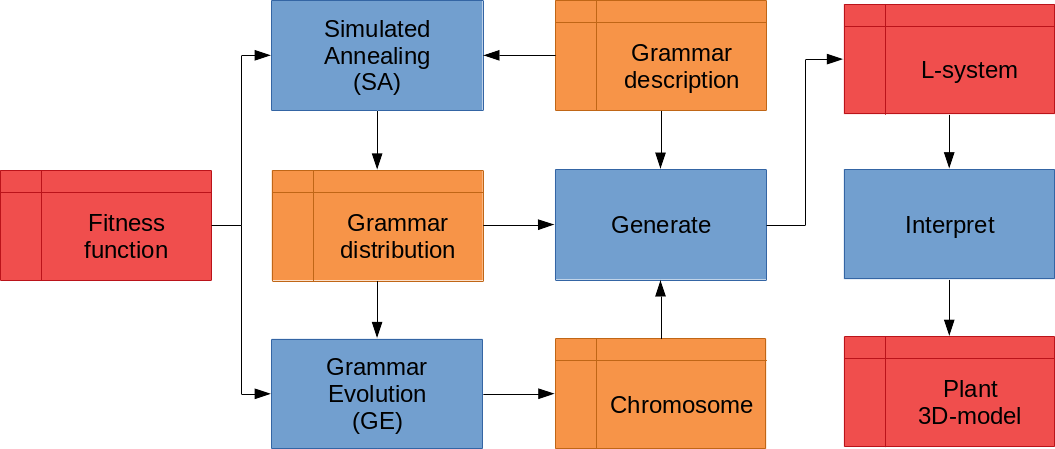
\includegraphics[width=1.0\textwidth]{figures/dgel}
    \caption[Overview of DGEL]{Overview of DGEL. Blue boxes represent processes. Red and orange boxes represent models. Orange boxes represent the models that define a unique L-system.}
    \label{fig:dgel}
\end{figure}

Figure~\ref{fig:dgel} illustrates the processes and models of the DGEL algorithm.
A plant 3D model is interpreted from an L-system.
The L-system is generated by a chromosome using a grammar distribution for a grammar description.
These three models: the grammar description, grammar distribution and the chromosome, together define the L-system.
All L-systems generated using the same grammar description, grammar distribution and chromosome will result in the exact same L-system, which also will be interpreted into the exact same plant 3D model.
GE is used to generated a good chromosome based on the grammar description, grammar distribution and a fitness function.
The grammar distribution is generated by Simulated Annealing (SA) based on the grammar description and a fitness function.
The fitness function models how aesthetically pleasing a plant is by assigning it score in range $[0, 1]$, where 0 is the worst, and 1 is the best.

\section{Representing an L-system with Grammar}
\label{sec:grammar}
As described, the L-systems in DGEL are represented by a chromosome, a grammar description and a grammar distribution.
If we assume a uniform grammar distribution, only a chromosome and a grammar description is required.

The grammar description, represented in a format such as the Backus Naur Form (BNF), describes the syntax of the L-system.
For example, it may describe that an L-system consists of a number of rules, each with a predecessor and successor, where a predecessor contains one character, etc.
The chromosome describes the choices to be made in the grammar description, for example how many rules there are, or which character the predecessor contains.
These choices are what creates the variations in the L-systems.
If there were no choices, there would only exist one single L-system.

This method of representing the L-systems was based on Beaumont and Stepneys's work on applying GE to plant L-systems~\cite{2009Beaumont}, in addition to Ortega et al.'s work on applying it to fractal L-systems~\cite{2003Ortega}, and Ryan et al.'s introduction of GE~\cite{1998Ryan}.

While Ortega et al.\ and Beaumont and Stepney make assumptions about the grammar to significantly simplify it and reduce the search space~\cite{2003Ortega, 2009Beaumont}, the DGEL method uses a grammar that covers the largest search space reasonably possible.
To make the search space reasonable, there still have to be some limits.
The number of productions, string length, and number of characters for a variable were limited to a maximum of 20.
A higher number did not seem reasonable as no L-systems in the literature reviewed used larger numbers, and the search times for higher numbers started to become unreasonable long.

Additionally, to limit the complexity of L-systems, complex features such as leaves, flowers, branch width and more were not included.
Thus the grammar used can only produce the branches of a plant.
This is the most essential part of a plant, which can be expanded later by modifying only the grammar description.
Listing~\ref{lst:grammar} shows the actual grammar description used during the development and testing of the algorithm, while Listing~\ref{lst:grammar2} shows a grammar description that supports leaves and varying branch width.

\begin{lstlisting}[caption=ABNF grammar description used in DGEL, label=lst:grammar, float]
lsystem = axiom productions
axiom = string
productions = 1*20production
production = predecessor successor
predecessor = variable
successor = string
string = 1*20(symbol / stack)
stack = "[" string "]"
symbol = variable / operation
variable = %x41-55
operation = "+" / "-" / "^" / "&" / ">" / "<"
\end{lstlisting}

\begin{lstlisting}[caption=ABNF grammar description supporting leaves and varying branch width, label=lst:grammar2, float]
lsystem = axiom productions
axiom = string
productions = 1*20production
production = predecessor successor
predecessor = variable
successor = string
string = 1*20(symbol / stack / leaf)
symbol = variable / operation
variable = %x41-55
operation = "+" / "-" / "^" / "&" / ">" / "<" / "!"
stack = "[" string "]"
leaf = "['{+f-f-f+|+f-f}]"
\end{lstlisting}

To be able to use different grammar distributions, the chromosome representation is a different from that of Ryan et al.\ where each gene is an unsigned 8-bit integer and the choice to be made is the alternative index by the gene modulo the number of alternatives~\cite{1998Ryan}.
Each gene is still represented by an unsigned integer, but it is 32-bit instead of 8-bit, and the interpretation of the integer is different.

A gene in the DGEL chromosome can be viewed as an index into the value range of the 32-bit integer.
This value range, from $0$ to $2^{32}$, can be viewed as a line with segments representing each alternative in a rule in the grammar.
In the case of a uniform distribution the segments would be equal in length, while for a different distribution the lengths will differ.
The value of each gene in the chromosome is randomly picked from a uniform distribution, thus making the actual distribution dependent on the grammar distribution.

Figure~\ref{fig:gene} illustrates an example of this process.
A choice is to be made between $C$, $D$, $E$ and $F$ in the rule $A \rightarrow C / D / E / F$.
A chromosome of length 4 containing 4, 3, 0 and 7 is used, and the next gene to be used in the chromosome is the second position, i.e.\ the value 3.
Each gene is a 3-bit unsigned integer, thus having 8 possible values in range $[0, 8)$.
Since there are four alternatives, and a uniform distribution is used, the 3-bit value range is split into four segments of 2 values.
The gene value 3 maps into the second segment, which maps to the second alternative in the rule, i.e.\ $D$.
This process would then continue with the next gene, 0, on the $D$ rule.

\begin{figure}
    \centering
    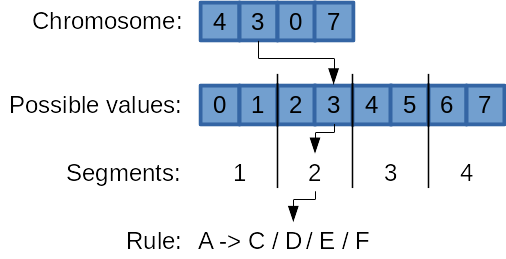
\includegraphics[width=0.8\textwidth]{figures/gene}
    \caption[Example grammar alternative selection from gene]{Example grammar alternative selection from gene. In the figure, the gene is a 3-bit integer, and thus has 8 possible values.}
    \label{fig:gene}
\end{figure}

\section{Interpreting L-systems Into Plant 3D Models}
As seen in Figure~\ref{fig:dgel}, after an L-system has been generated, it needs to be interpreted into a 3D-model such that people may see the plant.
Turtle interpretation is used to do this~\cite{2012Prusinkiewicz}, as it is a popular method used in the literature.
A 3D version of the turtle interpretation is used, where the turtle can draw lines with \textit{F}, and rotate around three axes using \textit{-} and \textit{+} for yaw, \textit{\textasciicircum} and \textit{\&} for pitch, and \textit{<} and \textit{>} for roll.
The bracket operators, \textit{[} and \textit{]}, are used to create branches.
Table~\ref{tab:turtle-cmd} shows a complete overview of the characters and their operations, including extra operators used for more control and features like leaves (e.g.\ Listing~\ref{lst:grammar2}).

\begin{table}
    \centering
    \begin{tabular}{| c | l |}
    \hline
    \textbf{Character} & \textbf{Operation} \\ \hline
    F & Draw line forward \\ \hline
    + & Yaw left \\ \hline
    - & Yaw right \\ \hline
    \textasciicircum & Pitch up \\ \hline
    \& & Pitch down \\ \hline
    < & Roll left \\ \hline
    > & Roll right \\ \hline
    | & Yaw 180° \\ \hline
    [ & Push state \\ \hline
    ] & Pop state \\ \hline
    \{ & Begin surface \\ \hline
    \} & End surface \\ \hline
    ! & Decrease width \\ \hline
    ` & Next color \\ \hline
    f & Draw line forward \\
    \hline
    \end{tabular}
    \caption[Turtle interpretation of L-system characters]{Turtle interpretation of L-system characters. \textit{f} does the same as \textit{F}, but is not allowed as a predecessor int the grammar such that it can not recurse.}
    \label{tab:turtle-cmd}
\end{table}

The actual 3D model created from this interpretation is kept as simple as possible while still trying to look somewhat natural.
The branches (created by the \textit{F} character) are brown stretched cubes.
Leaves are green flat surfaces.
An example can bee seen in Figure~\ref{fig:example-model}.

As a discrete L-system is used, the turtle interpretation requires some parameters that control the drawing.
While some evolutionary L-system techniques evolve the turtle interpretation parameters as well as the L-systems, to keep the process simple, DGEL does not.
Additionally, if the discrete L-system is swapped with a parametric L-systems, these parameters are no longer required.
The parameters used here were based on the 3D bush and 3D plant presented by Prusinkiewicz and Lindenmayer (s 1.25 and 1.26)~\cite{2012Prusinkiewicz}.
They can be seen in Table~\ref{tab:turtle-param}.

\begin{table}
    \centering
    \begin{tabular}{| l | l |}
    \hline
    \textbf{Parameter} & \textbf{Value} \\ \hline
    Width & 0.05 \\ \hline
    Angle & 22.5° \\ \hline
    Iterations & 5 \\ \hline
    Step & 0.2 \\
    \hline
    \end{tabular}
    \caption[]{Turtle interpretation parameters}
    \label{tab:turtle-param}
\end{table}

As described earlier, leaves and branches with varying widths are not included.
Without these, the plants may look ``dead'', and thus can not be very aesthetically pleasing.
To work around this widths of branches were heuristically set and leaves were heuristically placed.
These heuristics were based on observations of real plants and L-system based 3D models such as the aforementioned models presented by Prusinkiewicz and Lindenmayer (Figures 1.25 and 1.26)~\cite{2012Prusinkiewicz}.

The branch widths are determined by their distance from the leaf node of the branches.
From a leaf node, the branch width will increase by a fixed number towards the first branching point.
In a branching point, the width will be set to the largest of the outgoing branches.
Then, the width will continue to increase towards the root.
Thus the plant will have natural-looking branches that are larger closer to the root.
Bigger plants will naturally have thicker branches than smaller plants.

Leaves are placed from the branch nodes towards the root on each branch segment in increasing sizes, until they become too big.
Thus, the leaves a the edge of the branches are the smallest, and they get bigger towards the root.
To prevent thick branches, e.g.\ the trunk of a tree, to have leaves directly placed on them, the leaves will no longer be placed when they reach a specific size.
The leaves are always pitched upwards, with a random noise applied to the pitch to look more natural.
They have a random rotation around the branch.

This interpretation of the L-system can be swapped out with a different interpretation, while still using the DGEL algorithm.
For example a more realistic interpretation with smoothed branches or branches bent by gravity could be used.
Thus the DGEL algorithm is not dependent on this particular interpretation, but the results described later will be.

\section{Using a Grammar Distribution to Limit Search Space}
In DGEL, grammar distributions are used for three reasons: to guide the GE to more efficiently find good plants, to guide GE to search in a space with certain types of plants, and to prevent infinite recursion.

The distribution is a set of weights per choice per rule per depth, as illustrated in Figure~\ref{fig:distribution}.
The depth is the current branching depth of the L-system, controlled by the bracket operators, and defined as the \textit{stack} rule in the grammar in Listing~\ref{lst:grammar}.

The example figure shows a case where a choice is to be made between the alternatives C, D, E and F in rule $A \rightarrow *(C / D / E / F)$.
There are two different choices in the rule: selecting the number of repetitions (indicated by the asterisk character, \textit{*}), and selecting the C/D/E/F alternative.
In the example, the depth is 0 (no branching), the rule is $A$ and the choice is the second.
This maps to the weight array: $[0.1, 0.4, 0.3, 0.2]$ which should be applied to the C/D/E/F choice.
Thus, $C$ has a 10\% chance of being selected, $D$ has 40\%, $E$ has 30\%, and $F$ has 20\%.
These weights are then used to define the segments in the gene, as described in Section~\ref{sec:grammar}.

\begin{figure}
    \centering
    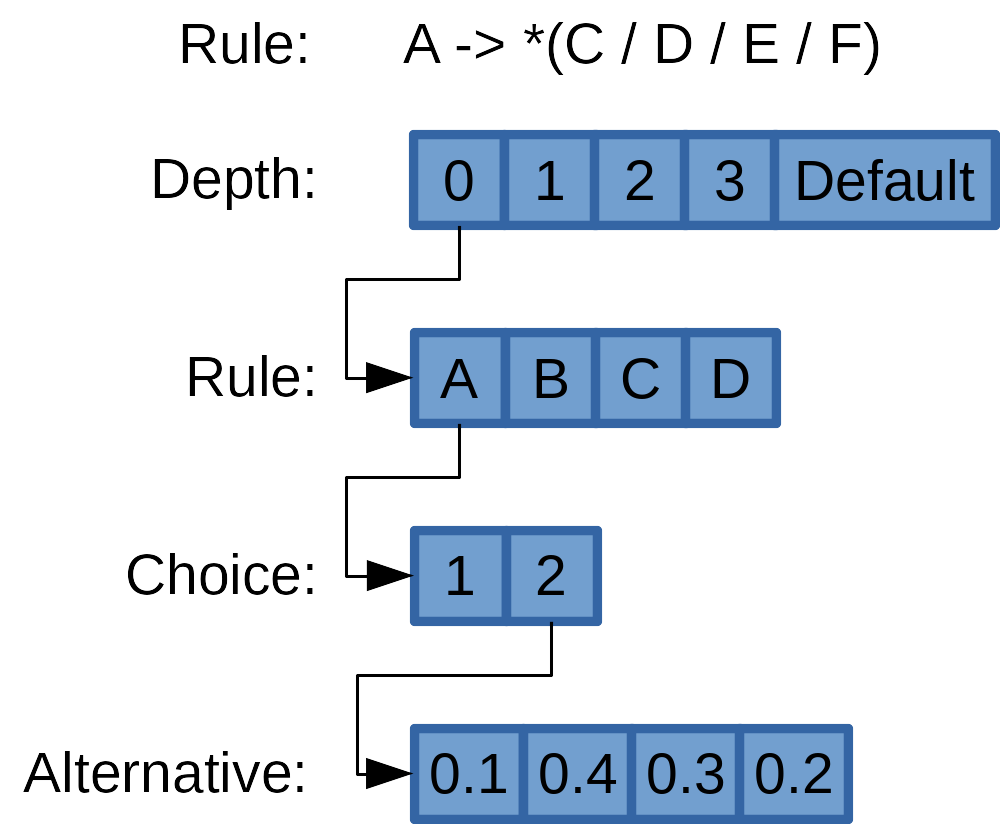
\includegraphics[width=0.6\textwidth]{figures/distribution}
    \caption[Example grammar distribution]{Example grammar distribution applied to the second choice of rule $A$ at depth 0.}
    \label{fig:distribution}
\end{figure}

By using a specialized distribution, rather than a uniform distribution, the generator may be targeted at specialized L-systems, or just have a higher average fitness score for the generated plants.
For example, the distribution may focus more on producing the \textit{F} character which is used for drawing the branches.
Or it may be focused on the \textit{stack} rule that produces branching points.
This may in turn increase the rate of produced plants that have long or many branches.

In addition to the distribution weights shown in Figure~\ref{fig:distribution}, there is a default distribution that will be used if there does not exist a mapping for a rule and choice at a specific depth.
This can be used to prevent infinite recursion with the \textit{stack} rule.
For example, the distribution for the grammar in Listing~\ref{lst:grammar} may specify the weights $[0.5, 0.5]$ for the second choice (\textit{symbol / stack}) in the \textit{string} rule at depth 0, 1 and 2, such that there is an equal change to produce a string and a stack (branching point).
To prevent any further branchings, the weights $[1.0, 0.0]$ may be specified for the default distribution, causing it to not produce a stack at depth 3 or deeper.

To find specialized distributions to more efficiently generate good plants or generate different types of plants, the weights in the distribution need to be optimized.
As the distribution maps from depth, to rule, to choice, to alternative (weight), it is a four-dimensional parameter space to be optimized.
DGEL uses Simulated Annealing (SA) to perform the optimization, but other multi-dimensional parameter optimizers could just as well be used.

Specifically, DGEL implements the basic SA approach~\cite{2000Ozdamar}, as described by Onbaşoğlu and Özdamar~\cite{2001Onbasoglu}.
The only difference is that the initial solution is not initialized randomly, but initialized from a pre-optimized solution, such that it has a better starting point.
In the DGEL SA, the \textit{solution} is the distribution itself, filled with weights for each of the alternatives in each of the choices in each of the rules in a limited set of depths.

A neighbour solution is generated in the same manner as Onbaşoğlu and Özdamar describes~\cite{2001Onbasoglu}: selecting one single random weight and either increasing or decreasing the weight randomly, bounded to the range $[0.0, 1.0]$ in the case of DGEL.
A key difference is that since these are \textit{weights}, the remaining weights in the same set of weights have to be modified such that the sum of all of the weights equal 1.
If the sum of the remaining weights is greater than 0, they can be scaled by a normalization factor, calculated by $\frac{(1 - w)}{(1 - w_0)}$, where $w$ is the new value of the modified weight, and $w_0$ is the old value of the modified weight.
If the sum of the remaining weights is exactly 0, scaling the weights will not work, as they would remain 0.
The alternative solution is to divide the ``remaining weight'' over the remaining weights.
This is done by setting the remaining weights to $\frac{(1 - w)}{(n - 1)}$, where $w$ is the new value of the modified weight, and $n$ is the number of weights.

Accepting a neighbour solution also follows the same approach as Onbaşoğlu and Özdamar describes~\cite{2001Onbasoglu}.
To do this, an $f(x)$, where $x$ is a grammar distribution, has to be defined.
The performance of a grammar distribution can not directly be measured, but it can be estimated by measuring the average performance of the L-systems it generates.
As the performance of the L-systems generated may vary by a big degree, the average performance, $mean$, is only accepted after a specified amount of L-systems, $n$, have been generated, and the standard error of the performance, $se$, is below a threshold value, $t$ (Algorithm~\ref{alg:eval-dist}).

\begin{algorithm}
\caption{Distribution evaluation}
\label{alg:eval-dist}
\begin{algorithmic}
\Function{evaluate\_dist}{$dist$, $n$, $t$}
    \State $samples\gets \Call{empty\_list}{}$
    \State $mean\gets UNDEFINED$
    \State $se\gets INFINITE$
    \While {$se\geq t$}
        \State $new\_samples\gets \Call{generate}{$n$, $dist$}$
        \State $samples\gets \Call{concat}{$samples$, $new\_samples$}$
        \State $mean\gets \Call{mean}{$samples$}$
        \State $se\gets \Call{standard\_error}{$samples$}$
    \EndWhile
    \State \Return $mean$
\EndFunction
\end{algorithmic}
\end{algorithm}

\section{Using Grammar Evolution to Search the Space}
The main component of DGEL is the Grammar Evolution (GE) of the L-systems, which is used to search the parameter space for the best L-system.
The GE process takes a grammar description and a grammar distribution as the input, and produces a single L-system chromosome as the output.

It follows the process as described by Ryan et al.~\cite{1998Ryan}, but with some modifications to the representation as described in Section~\ref{sec:grammar}.
Ryan et al.\ do not describe the selection strategy they used, while Beaumont and Stepney use a simple selection strategy where a percentage of the best individuals are selected as parents~\cite{2009Beaumont}.
Since GE is a specialization of GA, GE can use the same selection strategies as GA.
Thus, tournament selection was selected for DGEL, based on Blickle and Thiele's structured comparison of selection strategies~\cite{1995Blickle}, and Razali and Geraghty's comparison of selection strategies applied to the traveling salesman problem~\cite{2011Razali}.
Both tournament and ranking selection are recommended as good options, but tournament selection performs faster~\cite{1995Blickle}.
Thus because it is assumed that DGEL may be used in real-time applications, tournament selection is preferred.

To make the choice of tournament selection based on Blickle and Thiele's comparison to be valid, the GE algorithm is implemented as GA is described in the same paper.

\section{Using a Fitness Function to Evaluate Plants}
A crucial component of both the SA and GE process is the fitness function.
The fitness function is used by SA to evaluate the grammar distributions, and by GE to evaluate individual L-systems.
Its function is to evaluate how ``good'' the L-system plants are, or more specifically how ``aesthetically pleasing'' they are.
The literature on evolutionary L-systems generally aim the fitness function at evaluating how realistic the plants are by using metrics such as its light gathering ability, positive phototropism and structural stability.

It is assumed that a baseline for aesthetically pleasing plants is that they look at least somewhat realistic, otherwise they would not look like plants at all.
Thus, the metrics used for the fitness function in DGEL uses metrics from the literature, or metrics inspired from the literature, where the metrics usually are targeted towards realistic plants.
Additionally, the metrics were improved upon by generating a plants and looking for bad features in well-scored plants.
Table~\ref{tab:fitness} lists all of the metrics.

\begin{table}
    \centering
    \begin{tabularx}{\textwidth}{| l | X | l | l |}
    \hline
    \textbf{Metric} & \textbf{Description} & \textbf{Equation} & \textbf{Weight} \\
    \hline
    Nothing & Punish plants that have no branches (can not be seen) & \ref{eq:nothing} & 1 \\
    \hline
    Closeness & Punish plants with branches very close to each other & \ref{eq:closeness} & 1 \\
    \hline
    Drop & Punish plants based on how much the plant grows downwards & \ref{eq:drop} & 1 \\
    \hline
    Balance & Reward plants that have their center of gravity closer to their root & \ref{eq:balance} & 1 \\
    \hline
    Complexity & Reward plants with a balanced number of branches & \ref{eq:complexity} & 1 \\
    \hline
    Foliage & Reward plants with more leaves & \ref{eq:foliage} & 1.5 \\
    \hline
    Length & Reward longer plants & \ref{eq:length} & 1 \\
    \hline
    Curvature & Reward plants that have somewhat curving branches & \ref{eq:curvature} & 0.4 \\
    \hline
    \end{tabularx}
    \caption[]{Turtle interpretation parameters}
    \label{tab:turtle-param}
\end{table}

\textit{Nothing} is the simplest and most basic metric.
It punishes plants that have no branches.
This may happen if for example the L-system contains no drawing commands (the character \textit{F}).
Equation~\ref{eq:nothing} demonstrates this by giving it a score of -1 if it does not have any branches.
In this case no other metrics will make any difference.
The $branches$ function returns the number of branches.

\begin{equation}
\label{eq:nothing}
    nothing(x) =
    \begin{cases}
        0,& \text{if } branches(x) > 0  \\
        -1,& \text{otherwise}
    \end{cases}
\end{equation}

\textit{Closeness} is another punishing metric that punishes plants that have branches from the same branching point too close to each other.
The dot product between the direction of two branches is used for this metric.
The dot product is larger the closer the direction vectors are, becoming 1 when they are parallel.
If the largest dot product between branch directions in a branching point is below a threshold, $t$, there is no punishment.
Otherwise, the plant is punished by a factor depending on how much above the threshold the dot product is.
This factor is interpolated between 0 and 1 linearly from the threshold to 1.
Equation~\ref{eq:closeness} shows how the closeness is calculated.
The $closest$ function finds the closest dot product between branches in a branching point.
The threshold was experimentally set to 0.9 to punish plants that have branches that look like they clip into each other.

\begin{equation}
\label{eq:closeness}
    closeness(x) =
    \begin{cases}
        0,& \text{if } closest(x) < t \\
        -\frac{c - t}{(1 - t)},& \text{otherwise}
    \end{cases} \\
\end{equation}

\textit{Drop} is a third punishing metric that punishes plants that grow downwards.
It finds the lowest point on the plant, and punishes the plant if it is below 0.
Equation~\ref{eq:drop} demonstrates this.
The $lowestpoint$ function returns the smallest value of the y-component of all points on the plant.
This value is then clamped in the range -1 and 1 and interpolated using a sine function to quickly increase the punishment.
Thus plants where the lowest point is 0 or above will not be punished, while on plants where it is -1 or below will be punished by -1.

\begin{equation}
\label{eq:drop}
drop(x) = sin(clamp(lowestpoint(x), -1, 0) * \frac{\pi}{2})
\end{equation}

\textit{Balance} is a measure of how well balanced the weight of the plant is.
It is inspired by the Bilateral Symmetry measure by Ochoa where 2D plants that reach equally long both left and right are rewarded the most~\cite{1998Ochoa}.
A different approach has to be taken in 3D where there are not only two horizontal directions, but rather an infinite number.
The approach taken is to estimate where the center of gravity of the plant is, calculate the horizontal distance, $centerdistance$, to it, and compare it to how far the plant reaches, $centerspread$, in the horizontal direction of the center of gravity.
This is done by Equation~\ref{eq:balance}.
In the worst case, if both $centerdistance$ and $centerspread$ are the same, the plant will be punished by -1.
In the best case, if the $centerdistance$ is 0, i.e.\ the gravitational center is in the center of the plant, the plant will be rewarded by 1.
Since $centerdistance$ generally will increase with increasing $centerspread$, the plant will be more punished the more it spreads out in one direction.
Though by having most of it branches close to the root, it may mitigate the punishment.
Thus the fraction $\frac{centerdistance}{centerspread}$ is used.

\begin{equation}
\label{eq:balance}
balance(x) = (0.5 - \frac{centerdistance(x)}{centerspread(x)}) * 2
\end{equation}

\textit{Complexity} measures how complex the branching of the plant is.
It is inspired by the Structural Stability~\cite{1998Ochoa}, Plant Structural Stability~\cite{2009Corchado} and Proportion of Branching Points~\cite{1998Ochoa} measures.
These measures assume that the plant becomes too unstable to survive if it has too many branches growing from a branching point.
Corchado et al.\ additionally assume that plants with too few branches will have worse light gathering ability.
Thus there will be a sweet spot in the branching proportion which is rewarded the most.
If the proportion is too low or too high, the plant will be punished.
This is shown in Equation~\ref{eq:complexity} where if the branching proportion is below 1.2 (1.2 branches from a branching point on average), or above 5, it will be punished in range $[-1, 0]$.
While between 1.2 and 5, it will be rewarded in range $[0, 1]$.
The sweet spot is 2, where it will be rewarded by 1.
$icos$ interpolates the value from the first parameter, $a$, to the second parameter, $b$, using a cosine function.
The third parameter, $t$, is in range $[0, 1]$ and controls where between $a$ and $b$ the interpolation is.
This creates a smooth curve between the limits.

\begin{equation}
\label{eq:complexity}
\begin{aligned}
    complexity(x) =
    \begin{cases}
        -1, & b < 1 \\
        icos(-1, 0, \frac{b - 1.0}{0.2}), & b < 1.2 \\
        icos(0, 1, \frac{b - 1.2}{0.8}), & b < 2 \\
        1, & b < 3 \\
        icos(1, -1, \frac{b - 3}{5.8}), & b < 7 \\
        -1, & \text{otherwise}
    \end{cases}, \\
    \text{where } b = \frac{branches(x)}{branchings(x)}
\end{aligned}
\end{equation}

\textit{Foliage} measures how many leaves a plant has.
It is the main metric for measuring the light gathering ability of the plant, and is inspired by Ochoa~\cite{1998Ochoa}, Ebner~\cite{2003Ebner}, and Corchado et al.'s~\cite{2009Corchado} light gathering ability metrics.
The main point is that more leaves exposed to sunlight means that the plant has a better ability to survive.
For simplicity, the metric used in DGEL is based on Corchado et al.'s metric which simply rewards plants with more leaves~\cite{2009Corchado}.
It also counts leaves that are shadowed by other leaves, even though in reality these would gather only minimal amounts of light.
This selection of method was due to time constraints, and a more complex method like Ebner's would be better.
The metric used starts with a reward of 0 for 0 leaves and is asymptotic towards 1 when the leaf count, found by $leaves$, increases towards $\infty$.
Equation~\ref{eq:foliage} demonstrates this.
The $s$ constant controls how fast it should increase towards 1.

\begin{equation}
\label{eq:foliage}
    foliage(x) = \frac{leaves(x) * s}{1 + leaves(x) * s}, \text{where } s = 0.1
\end{equation}

\textit{Length} rewards plants that are longer.
It is inspired by Ochoa and Corchado et al.'s Positive Phototropism metrics where the assumption is that plants grow towards the sunlight and thus taller plants are better at surviving.
While Positive Phototropism only cares about the height of the plant, Length cares about how long the plant is, not considering if it grows upwards or not.
This change is made on the assumption that plants can gather more light both by growing upwards (cover more vertical area) and sideways (cover more horizontal area).
Additionally it was found during an early experiment that short plants were generally found as displeasing.
Like the Foliage metric, the Length metric is asymptotic towards 1 as the plant length increases towards $\infty$.
This is shown in Equation~\ref{eq:length}.
The length of the plant is found using $longest$, which finds the longest path in the branches of the plant from root to leaf and returns the number of segments in it.
As with the Foliage metric, the $s$ constant controls how fast it should increase towards 1.

\begin{equation}
\label{eq:length}
    length(x) = \frac{longest(x) * s}{1 + length(x) * s}, \text{where } s = 0.5
\end{equation}

\textit{Curvature} is a metric that rewards plants with more curved branches.
It was developed from the results of the first experiment where it was found that plants that looked ``static'' or ``stragith'' were not as pleasing as plants that looked more ``dynamic'' or ``curvy''.
As Equation~\ref{eq:curvature} demonstrates, the plant is rewarded more if the branch segments are oriented with a small angle different from their parent.
If the angle is too sharp, the plant is rewarded less, as the plant may look like ``doodles'' with such angles.
A sweet spot of 0.24711092, which is rewarded by 1, was found to provide a good curvature in the plant.

\begin{equation}
\label{eq:curvature}
\begin{aligned}
     a = avg(minangles(x))  \\
     min = 0  \\
     opt = 0.24711092  \\
     max = \frac{\pi}{4}  \\
     f(x) =
    \begin{cases}
        icos(0, 1, \frac{a - min}{opt - min}), & a >= min \text{ and } a < opt \\
        icos(1, 0, \frac{a - opt}{max - opt}), & a >= opt \text{ and } a < max \\
        min, & \text{otherwise}
    \end{cases}
\end{aligned}
\end{equation}

\chapter{Evaluation of Algorithm}

\section{Experiment Setup}

\section{Results}
% !TEX root = ../Masters.tex
\chapter{Discussion}

\chapter{Related Work}
Xueqiang and Hong developed a generalized L-system method, called GLSM, that better follows botanical principles and increases the expressive ability of L-systems~\cite{2012Xueqiang}.
They emphasize the importance of a stochastic property in the L-systems to reflect botanical principles.

Wensheng and Xinyan model grass with stochastic L-systems and trees with parametric L-systems~\cite{2010Wensheng}.
For the tree models, they create one L-system where four parameters determine the branching angles and branch lengths.
They show how two different set of parameter in the same L-system can generate two different looking trees, and how adding stochastic multiples to the parameters can generate more naturally looking trees.
This is different from stochastic L-systems, because here they multiply stochastic values with parameters in the productions, while stochastic L-systems select productions stochastically.

%Niklas pioneered artificial evolution of L-systems in 1986. % Can't find copy of paper. Only have one source from another paper. Remove this?
Jacob argues that manually inferring an L-system from a real plant seen in nature is a difficult and tedious task involving several steps~\cite{1994Jacob}.
Some of these steps can be automated using evolutionary algorithms, specifically defining L-systems, comparing the generated plant with the real plant and correcting the L-system based on how it matched.
Based on this, Jacob defines three parts of evolutionary L-system inference: generation functions that create L-systems within some constraints, evaluation functions that measure the fitness of the interpreted L-system, and modification and selection functions that allow editing of L-systems with evolutionary techniques.

To evolve the L-systems, Jacob uses Genetic Programming (GP) techniques introduced by Koza~\cite{1992Koza}.
The difference is that Jacob uses higher-order building blocks for generation and modification of expressions.
A pool of expression patterns is defined that contains several expressions that each are represented in a tree structure.
Expressions can be combined using pattern matching, such that if a leaf node of an expression matches a root node of another expression, they can be combined.
Thus, an L-systems may be built by plugging together expressions in various ways, and the resulting L-system is always guaranteed to be valid.

Jacob defines multiple genetic operators, such as mutation and crossover.
Mutation replaces a subterm of an expression with another equivalent subexpression.
Crossover exchanges to subexpressions between two parents.
Both operators use pattern matching to find subexpressions in the L-system that can be modified.
Multiple patterns may be defined for each operator and are ranked such that if there is a match with multiple patterns, the one with the highest rank is selected.

The technique described by Jacob is shown to evolve a 3D L-system based on requirements that it should have a complex structure and leaves within a certain cubic boundary.
Jacob took this method further and showed that it could evolve L-systems that looked more like plants with certain requirements~\cite{1995Jacob,1996Jacob,1996Jacob-2}.

Mock continues Jacob's work, but works directly with L-system strings instead of expressions~\cite{1998Mock}.
It is thus more of a Genetic Algorithm (GA) technique rather than a GP technique.
The L-systems used are simple 2D interpreted L-systems that only have one node rewriting rule with branching.
The successor of this single rule is used as the genetic representation in the genetic algorithm.
Two genetic operators are used: crossover and mutation.
Crossover finds a random substring in each parent with equal number of branching brackets and exchanges them.
Mutation also finds a random substring the same way, but replaces it with a new randomly generated string instead.
To select individuals from the population that should be used for the next population, both humans and a fitness function have been used independently.
Humans manually assigned fitness to the phenotypes and selected one individual to keep.
When using humans, the generated L-systems started as weed-like or random doodles and ended up with simple 2D plants.
The fitness used was a simple ``tall and wide plants preferred'' function that ended up generating objects that looked less like pants than the human-selected samples.

Ashlock et al.\ use an evolutionary algorithm to evolve both the grammar and the interpreter parameters at the same time~\cite{2006Ashlock}.
This resulted in a larger variety of generated plants.
They pack the grammar and interpreter parameters as real parameters, which made it possible to solve it as a real parameter optimization problem.

Corchado et al.\ use genetic algorithms to grow plants over time, as they argue that L-systems alone inefficiently simulate growth and change over time~\cite{2009Corchado}.
They define the genotype as a compact string representation of a production rule, and the phenotype as the visualized plant.
The contact string representation consists of the predecessor and the successor connected by the ``='' character.
E.g.\ the production $F\rightarrow FF$ would be the string ``F=FF''.
Crossover is performed by selecting two strings based on their fitness and swapping two substrings between the two strings.
They mutate the string in two different ways: either by randomly changing a character in the string with another, or randomly changing a substring in the string with another.
The crossover and mutation needs to ensure that the string is still syntactically correct.
This mainly involves making sure the branching brackets always have a matching start and end bracket.
To solve this, they use Mock's solution~\cite{1998Mock}, where they only select strings with a balanced number of start and end brackets, which may also be zero brackets.

Beaumont and Stepney use Grammatical Evolution (GE) on L-systems to evolve them~\cite{2009Beaumont}.
GE is ``an evolutionary algorithm (EA) that can evolve complete programs in an arbitrary language using a variable-length binary string''~\cite{2003Oneil}.
Beaumont and Stepney do crossover by selecting random parents and selecting a random crossover point.
The crossover point is different for each parent, to allow variation in genome length in the children.
Elitism is used to allow the most fit genomes to pass to the next generation without being mutated.
They find that elitism is a significant advantage and that certain alterations to the grammar have a significant effect.

% !TEX root = ../Masters.tex
\chapter{Conclusion}

\section{Main Findings}

\section{Future Work}


\ifthenelse{\boolean{HarvardCitations}}{%
	\bibliographystyle{agsm} % used for Harvard style references. Names - Humanities & Interaction Design
}{%
	\bibliographystyle{ntnuthesis/ntnuthesis} %used for Vancover style references. Numbers - Computer Science & Physics
}

\bibliography{Masters}

\appendix
\include{appendix}

\end{document}
